\documentclass[12pt]{report}

\usepackage{graphicx}
\usepackage[margin=0.5in]{geometry}
\usepackage[utf8]{inputenc}
\usepackage{changepage}
\usepackage{amssymb,amsthm,amsmath,bm}

\newtheoremstyle{break}
  {\topsep}{\topsep}%
  {\itshape}{}%
  {\bfseries}{}%
  {\newline}{}%
\theoremstyle{break}
\newtheorem{defn}{Definition}

\begin{document}
%Titlepage
\newgeometry{margin=1.25in}
\begin{titlepage}

\begin{center}
	
\includegraphics[scale=1.25]{logo.pdf}
	\hspace{1cm}
	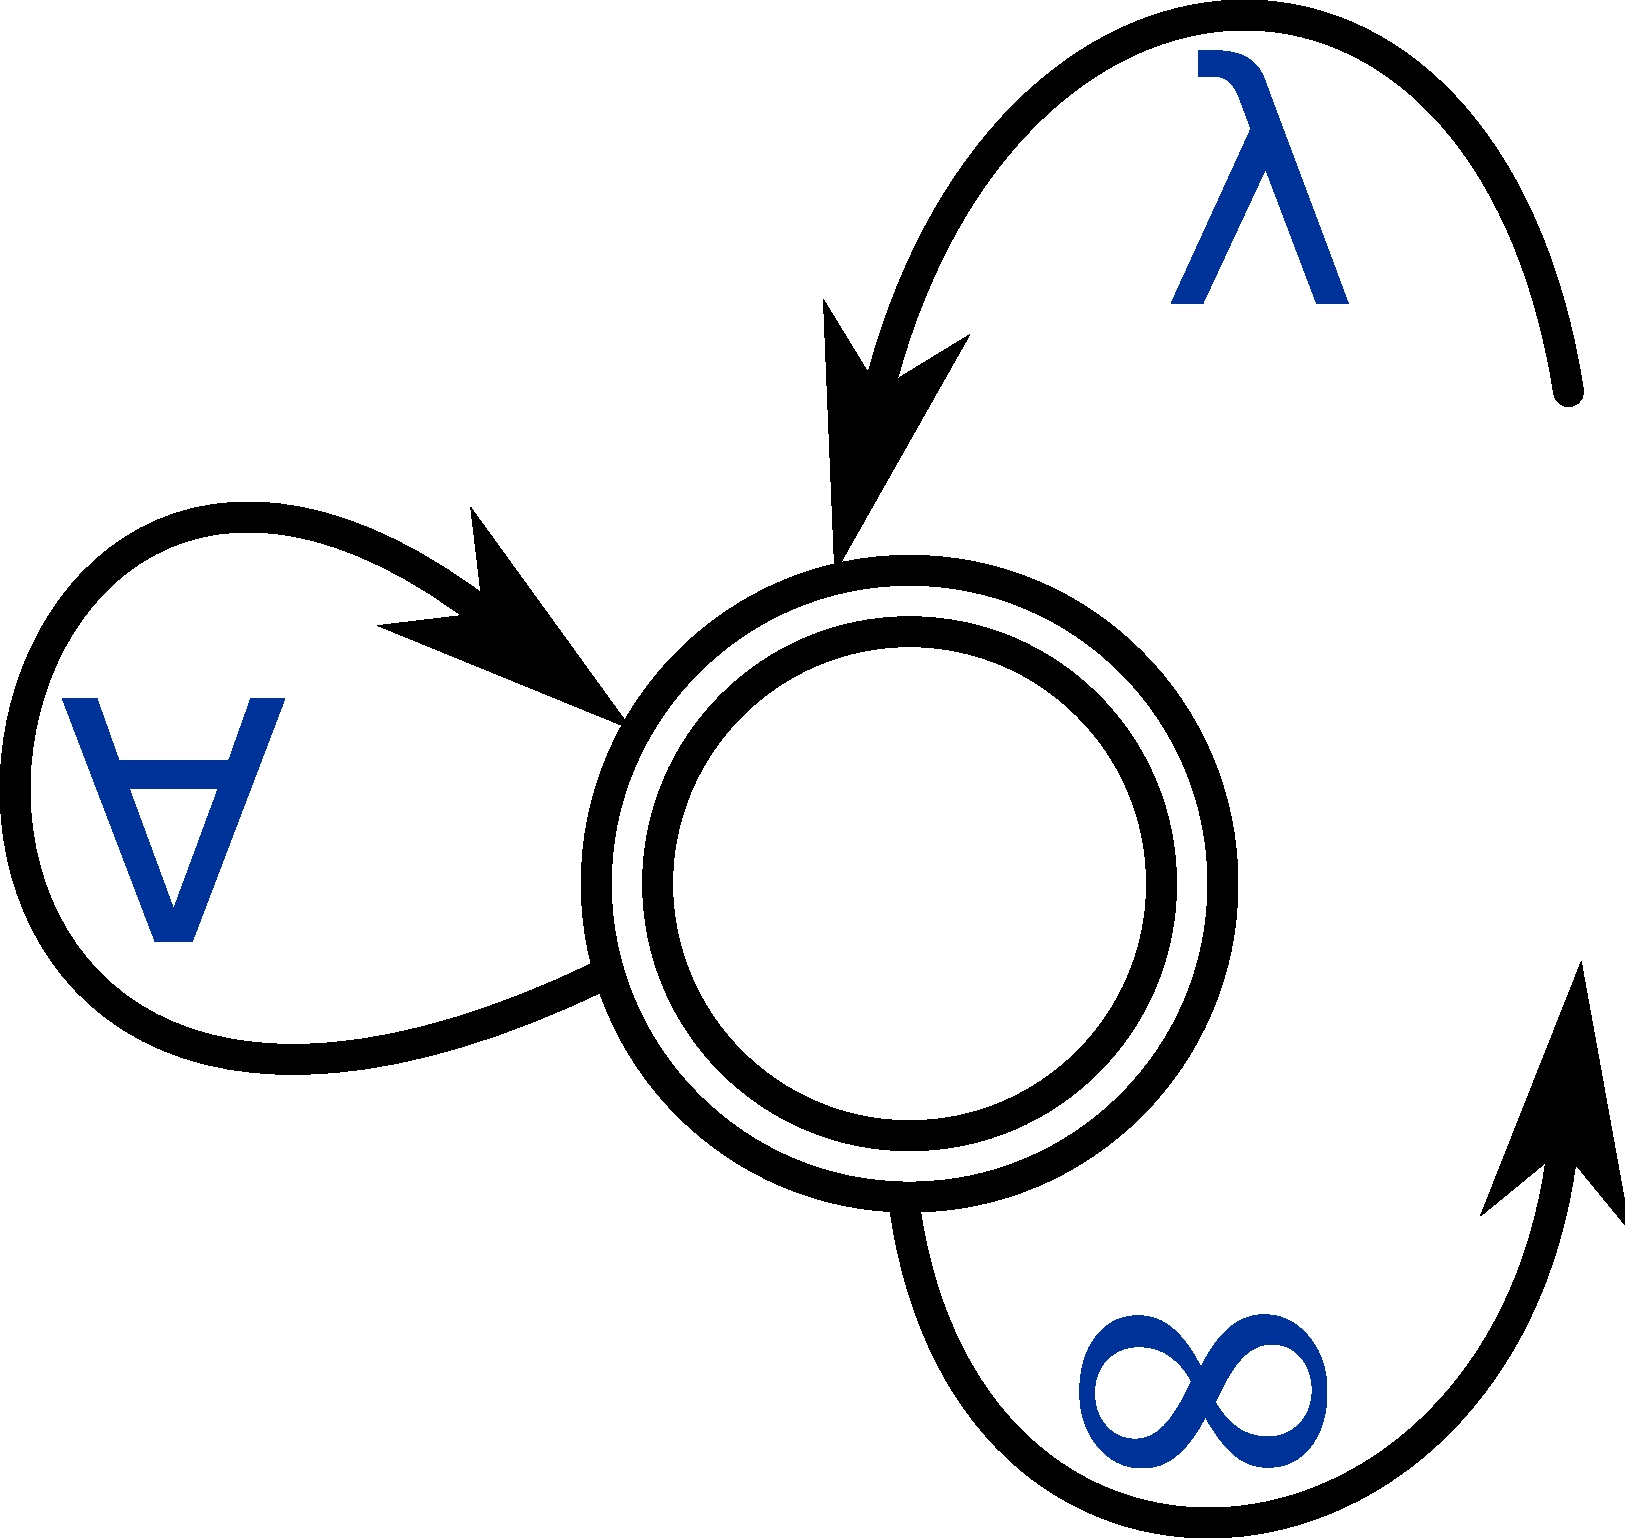
\includegraphics[scale=0.15]{logo.jpg}
	\vspace{2cm}\\
	
	%title
	\Huge \textbf{Argumentation Theory}\\ \large \textbf{Nonmonotonic Reasoning}\\
	\vspace{2cm}
	{\large \textbf{BACHELOR'S THESIS}} \vspace{2.5mm}\\ {\small submitted in partial fulfillment of the requirements for the degree of} \vspace{2.5mm}\\ 
	{\large \textbf{Bachelor of Science}} \vspace{2.5mm}\\ {\small in} \vspace{2.5mm}\\ {\large Software- and Information Engineering} \vspace{2.5mm}\\
	{\small by} \vspace{2.5mm}\\
	%author
	\huge \textbf{Christoph Groß, 1025119}\\
\end{center}
	%advisor
	\vspace{2cm}
\begin{flushleft}
	\begin{adjustwidth}{-0.5in}{}
	{\small to the Faculty of Informatics \\ at the Vienna University of Technology \vspace{2.5mm}\\ Advisor: Ao.Prof.Dipl.-Ing.Dr.techn. Christian Georg Fermüller}
	\end{adjustwidth}
\end{flushleft}

\end{titlepage}
\restoregeometry{}

%Table of Contents
\tableofcontents{}

%Statutory Declaration
\chapter*{Statutory Declaration}
\addcontentsline{toc}{chapter}{Statutory Declaration}

Hereby I assure that this thesis is a result of my personal work and that no other than the indicated aids have been used for its completion.\\
Furthermore I assure that all the quotations and statements, that have been inferred literally or in a general manner from published or unpublished writings, are marked as such.\\
Beyond this I assure that the work has not been used, neither completely nor in parts, to pass any previous examination.

\vspace{1.5cm}
Vienna, \today
\hspace{1.5cm}
\begin{tabular}{l}
\makebox[2.5in]{\hrulefill}\\
Christoph Groß\\
\end{tabular}


%Acknowledgements
\chapter*{Acknowledgements}
\addcontentsline{toc}{chapter}{Acknowledgements}


%Abstract
\chapter*{Abstract}
\addcontentsline{toc}{chapter}{Abstract}

Throughout this thesis, I am going to explore the applications of argumentation theory in the context of nonmonotonic reasoning.\\
First off, I will introduce the necessary formal definitions, give a few easy examples as clarification and draw the theoretical conclusions.\\
In the next step, the reader is given an overview over the real-life applications of argumentation theory.\\
Finally I will append the documentation of an application specifically written during the course of this thesis, which purpose is to graphically help understanding the subject.\\

%Indentation/Skip for text
\setlength{\parindent}{0pt}
\setlength{\parskip}{1em}

%Chapter 1, Introduction
\chapter{Introduction}

%Nonmonotonic reasoning
\section{Nonmonotonic Reasoning}
\begin{flushleft}
When talking about nonmonotonic reasoning, one is referring to the process of deducing knowledge within a formal logic,
whose consequence relation does not fulfill the requirements of monotonicity.
%Definition of Monotonicity :TODO evtl. noch ein bsp. einbauen? auf default logic verweisen?
\begin{defn}[Monotonicity]
If for a given set of formulas $\bm{\psi}$ and a formula $\bm{A}$ the logical consequence $\bm{\psi \vdash A}$ holds, then $\bm{\psi,B \vdash A}$ still holds.
\end{defn}
As one can see, nonmonotonic sets of formulas might change their deducable knowledge as new facts are added. 
\end{flushleft}

\section{Argumentation Theory}
\begin{flushleft}
In a human context, we (hopefully) argue to reach a sound conclusion. We do that by claiming statements based on premisses, and usually, due to different perception and other factors,
these statements tend to vary in their degree of believability.

Argumentation Theory, from a logical point of view, tries to formalize these strategies and introduces rules to that purpose. 
Most of the definitions in this thesis were originally introduced in \cite{Dung}
\end{flushleft}






%Bibliography - references to papers
\begin{thebibliography}{1}
	\bibitem[Dung]{Dung} "On the acceptability of arguments and its fundamental role in nonmonotonic reasoning,...";\\Phan Minh Dung; 1995
	\bibitem[EgGaWo]{Egly} "Answer-Set Programming Encodings for Argumentation Frameworks"; Uwe Egly, Alice Gaggl, Stefan Woltran; 2010  
\end{thebibliography}

\end{document}





















